\label{sec:gui}

The interface might not be a very important topic in this project, however since we were 6 people put together in this group, not everyone could do the main tasks.

\subsection{First layout}

In the very beginning the idea was we wanted to throw magnetic darts at a shooting disc in front of the table. 
The idea was to have two cameras, one on the table and one pointing outwards and with that shoot out. 
Since we had a raspberry pi in the last project as a server, we thought, we might have it too in this project and hence we began developing a website in PHP.
A PHP server could use http protocols to display a user interface on any device and also it could communicate with a c++ script on the same machine. I have developed alot of websites in HTML/CSS/JS/PHP so it came as a first choice.

On top of the framework, i have used another sockets to provide the videofeed from the gantry to the website. This makes it possible to pick a target manually instead of automaticly. This is smart for testing.
This feature is directly correlated with the idea of magnetic darts and a wish to select the targets ourself in the beginning. 

To begin with, the website was a controlpanel with arrows on the left and the videofeed on the right. The arrows in the controlpanel was the only way to control the seight, but later i made it possible just to press on the video feed and select a target that way.

The design is taken from another website i have build and changed to fit this purpose. 
It is build from "Bootstrap", which is a css framework, that makes it a whole lot easier to develop an astetic looking website. 
Bootstrap was created at Twitter in 2011 and acts today as a leading framework for webdesigners, providing both features in CSS, javascript and icons.

As the project was delivered to us, it became aparent that we would not use a server to run the robot. That meant that the PHP script was pretty much unusable. 
Because so much work was put into it, we would not tear it all down, but instead use a ftp-socket on our PCs to display as a HTTP server. 
That would also make it possible to create an interface locally on your own pc. 

Another idea, was to use a QWebEngineView inside the Qt application. - Which is a browser within the application. This is like a frame in html.
This was a very nice idea. It would both make it possible to keep the Bootstrap CSS stylesheets standards, 
but because the QWebEngineView simply lacked css features and generally lacked, we returned to browser view.

Besides the fact that the work already had been done, There are other upsides to using the browser over an application:
\begin{itemize}
    \item The browser is made for graphical interfaces - It makes it alot easier to make it the way you want it. Easier design.
    \item You can play with alot of different features like shadows, z-height and kinds of different features of css
    \item The video socket would be easier to display through the browser though we would not need the socket if we chose the application alone.
    \item I did know how to attack this from the beginning
    \item Slower than application alone
\end{itemize}
Actually it is so easy to create a user interface via HTML/CSS/JS that Qt design uses what they call QSS - which is similar to CSS. 
Another thing is Qt use an XML format for designing, this too is much alike browsers html. But it is alot more complicated. Not meant for writing it yourself.
That means, that I would properly be able to design something, that would be quite similar it would just take alot more time. So what would be the difference?
A Qt widget would have:
\begin{itemize}
    \item Easier implementation. You do not have to create special signals forward and backward to create your implementation. Those are already made for you
    \item The code would be alot simpler to understand from whithin. It would all be in c++ and Qt design.
    \item The video feed would not need a socket at all, but could be displayed directly.
    \item The code would run faster and save memory.
    \item Lack of bootstrap features - meaning i would need to redesign it from scratch. Bootstrap really saved me some time designing.
\end{itemize}

To sum it down, it is alot easier to create the design and there is more features natively, but it comes at the price of speed and complexity in the code when others have to read.

\subsection{Final layout}
We had decided not to throw darts or at least wait until we had thrown something else and seen what the robot could do. That meant the design with the arrows was becomming a little unusable.
To move forward, a proposition to add new buttons to the controlpanel, which could actually control the robot, was given.
After a little designconsideration, a new design was made.

The design mimics the interface on the UR robot. It takes in both controls of the UR and the gribber. Adds a list and sends it to the tread that controls the robot. 
I've explicitly made it a list, like "linked list" in java, to make it problemfree to remove elements in the middle.

To finalize the layout we have also added icons and taskbar features, so that you can close and open the website without having to restart the program.

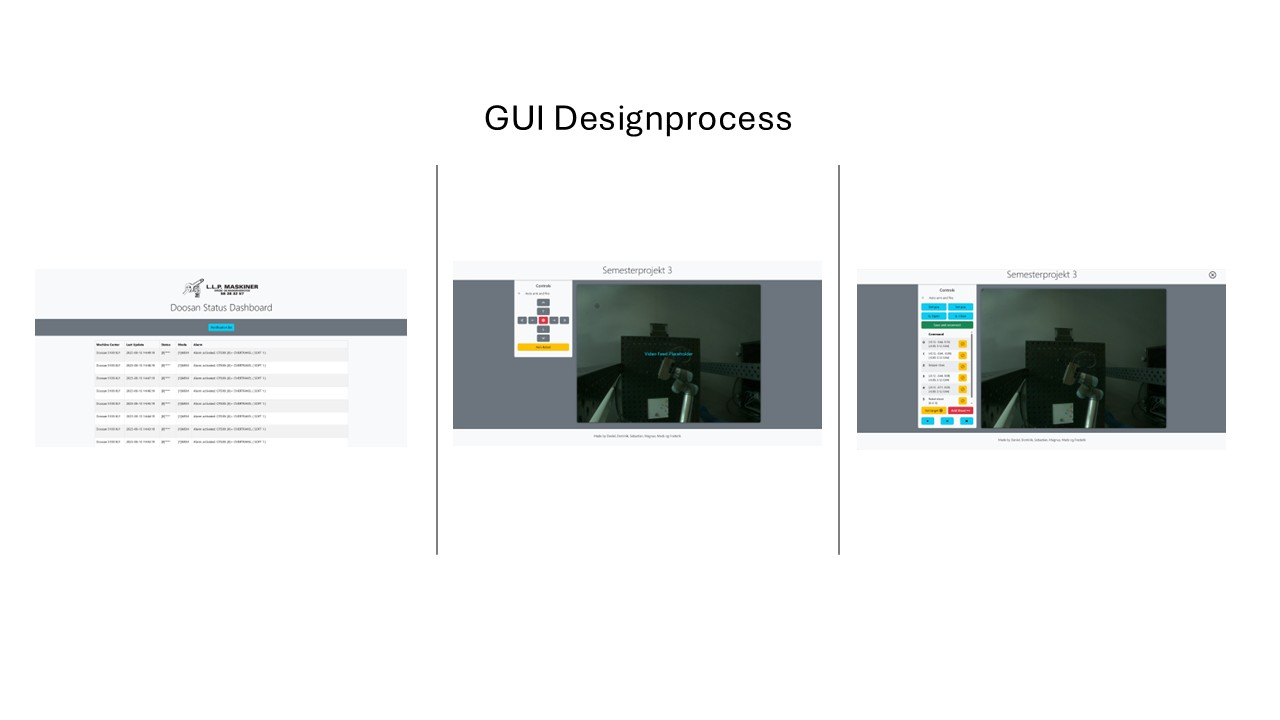
\includegraphics[width=190mm,center]{figures/GUI designprocess.jpg}

Later when we got the automatic functions up and running(The pick up ball function and the find box function)), the grapics changed somewhat. Instead of you had to click the target and then click set position, it was automaticly made to set position, so we could free up a button.
That meant we could add find ball in manual mode. So here the only difference was you had to pick your target yourself. This is also used heavily in the tests.

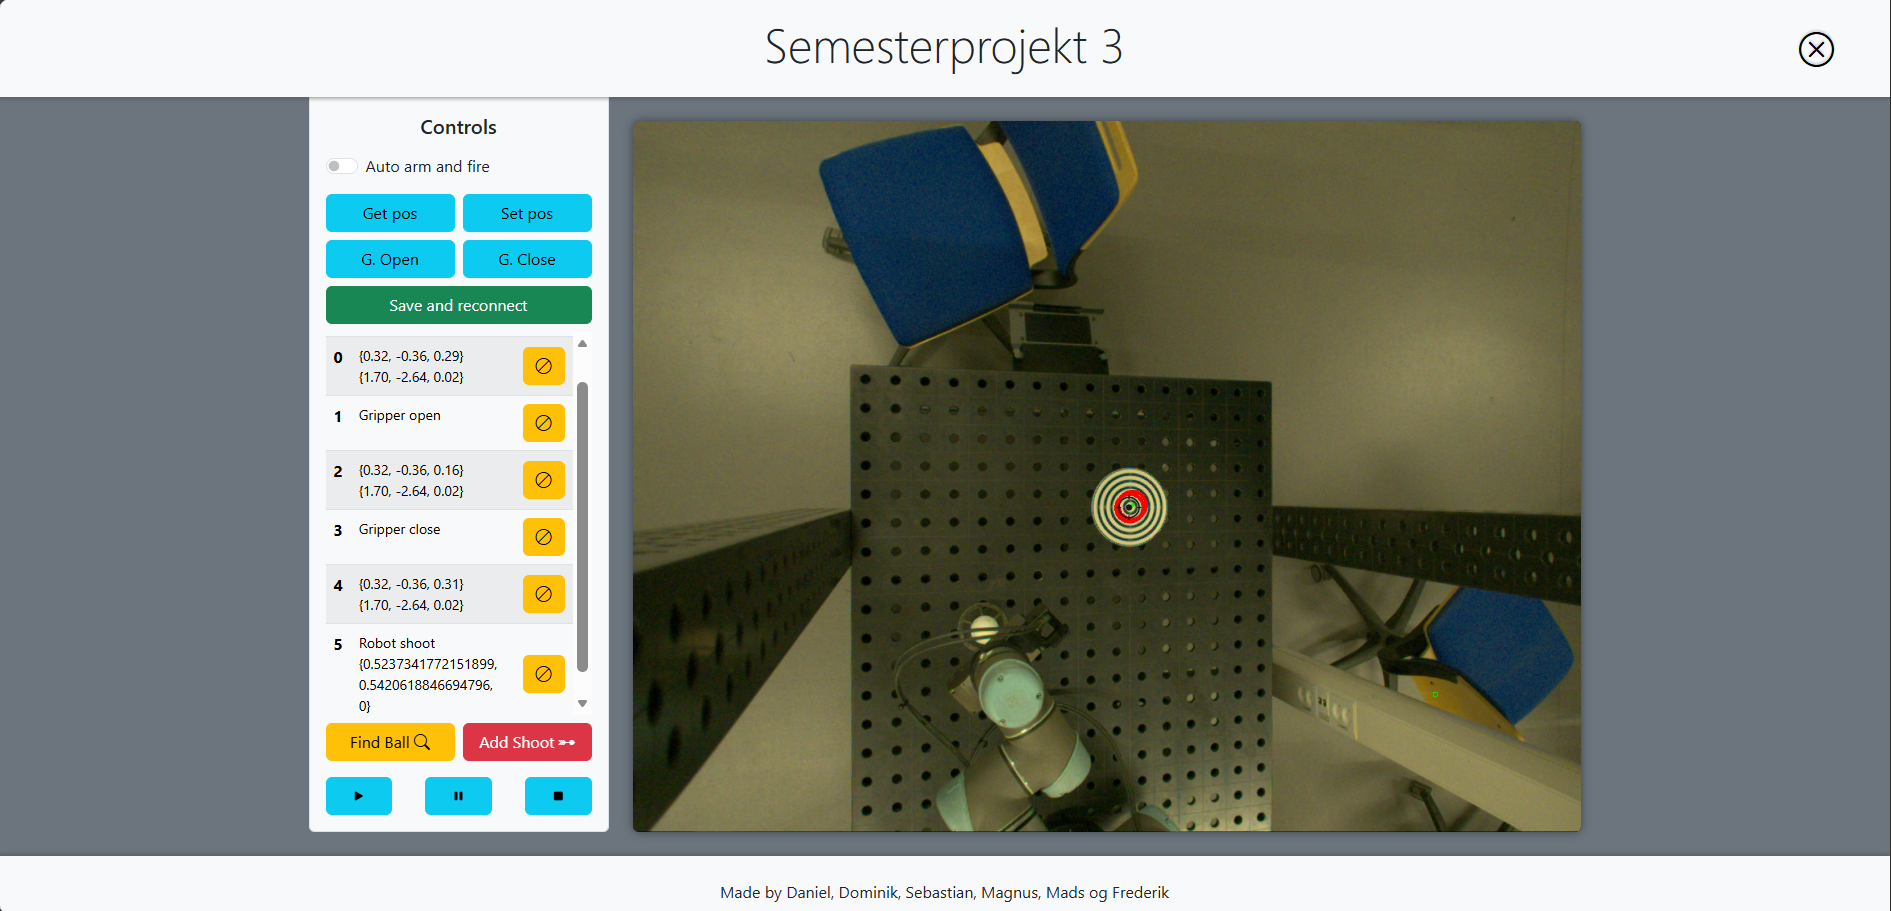
\includegraphics[width=190mm,center]{figures/GUI finalDesign.png}



